\chapter{Analisi dinamica}
Per analisi dinamica di un malware si intende lo studio di tutti i suoi comportamenti durante l'esecuzione in un ambiente controllato, come una sandbox.
Comportamenti sospetti possono essere la modifica di particolari chiavi di registri, la sovrascrittura di file privati dell'utente che non dovrebbe manipolare, la ricerca di file con nomi che potrebbero nascondere contenuti sensibili (ad esempio legge tutti i file che contengono la parola  "password" nel nome, come \texttt{password.txt}) o altre situazioni ancora.

Lo scopo di ciò che verrà realizzato in questa fase del progetto è di analizzare automaticamente l'esecuzione di un malware, così da riportare tutti gli elementi degni di nota all'analista o al servizio di Threat Intelligence in un formato machine-readable come JSON.
Le operazioni svolte in questa fase sono indipendenti dalla componente statica appena vista:
infatti, l'obiettivo sarà di lasciare la decisione all'analista o alla Threat Intelligence automatica sulla base di una confidence del risultato finale (se malevolo o meno), per eseguire questo processo solo nei casi di reale utilità, siccome sarà molto più esoso di risorse, quindi avente un maggior costo economico.

L'analizzatore dinamico, comprensivo della sandbox e di tutto ciò che è descritto in questo capitolo, è stato sviluppato ed eseguito in locale. Tuttavia, è già stato predisposto per un futuro impiego su un server gestito dall'azienda dove possa eseguire e ricevere task attraverso una REST API o altro interfacciamento.
Come nell'analizzatore statico, ritroviamo anche qui tutte le caratteristiche di qualità come la massima flessibilità ed estensibilità con altri strumenti nel corso della sua evoluzione.

L'esecuzione del possibile malware deve avvenire necessariamente in un ambiente isolato e supervisionato, idealmente riducendo a zero le possibilità che possa evadere e infettare il sistema host.
Non potrà mai esistere un sistema che, in maniera assoluta, permetta l'esecuzione di un programma senza rischi, potendo esistere vulnerabilità zero-day in tutte le componenti coinvolte, senza imporre limitazioni che inficerebbero sull'esito dell'analisi stessa, come disconnettere fisicamente un host reale da tutte le interfacce di rete e distruggere l'ambiente completamente.
Un software predisposto per fare ciò prende il nome di \emph{Sandbox}.

\section{Cuckoo Sandbox}
Per la realizzazione del progetto è stato adottato \emph{Cuckoo Sandbox}.
\footnote{\url{https://github.com/cuckoosandbox/cuckoo}}
Si tratta di un progetto open-source, rilasciato sotto licenza GPLv3 dalla Cuckoo Foundation, leader del settore che fornisce la base su cui lavorare e fare tutte le dovute modifiche del caso.
Consente di venire a conoscenza dell'esatto comportamento adottato dal malware durante la sua esecuzione, includendo la lista completa delle chiamate di sistema di ogni processo, nonché la cattura del traffico di rete, screenshot della UI durante l'esecuzione e il contenuto dei file creati nel sistema.

Viene fornito di due componenti: l'\emph{Host} e uno o più \emph{Guest}.
L'Host, anche chiamato Orchestrator, ha il compito di gestire i Guest, come avviarli, interromperli, analizzare il traffico di rete intercettato e tutta l'interpretazione dei risultati raw ottenuti dal Guest, così da ottenere il report.
Un Guest è tipicamente una VM, ma può essere anche un host fisico distinto, che contiene il sistema operativo, tutti i software che ci aspetteremmo in un PC tradizionale che vogliamo simulare, insieme all'Agent di Cuckoo, che comunicherà con l'Orchestrator per coordinare il lavoro e riportare i risultati.

\begin{figure}[htbp]
    \centering
    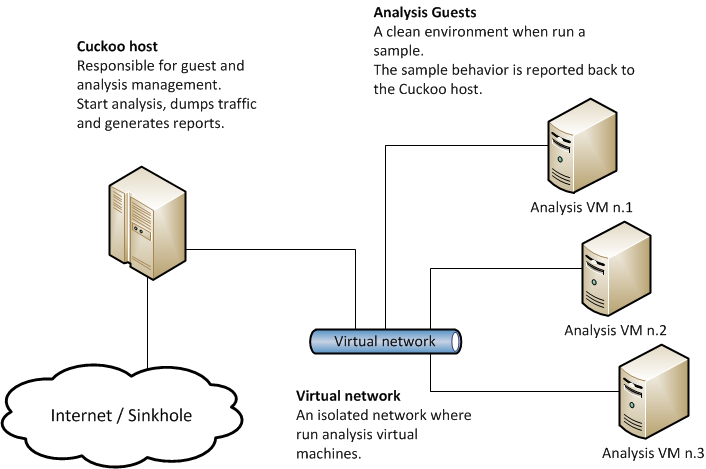
\includegraphics[width=0.9\textwidth]{assets/cuckoo_default_architecture.png}
    \caption{Architettura di Host e Guest di Cuckoo così come viene fornito}
    \label{fig:cuckoo_default_architecture}
\end{figure}

Su questa base, sono state fatte numerose lavorazioni illustrate nelle sezioni successive di questo documento. Non meno importante, è stata eseguita tutta l'installazione, configurazione su misura e hardening.

\section{Architettura realizzata}
L'architettura finale che è stata realizzata, e che verrà dettagliata di seguito, si compone come in figura \ref{fig:cuckoo_vms_architecture}.
Sono presenti diverse macchine virtuali:
\begin{itemize}
    \item \emph{Cuckoo Ubuntu VM} è l'Host, ossia dove risiede la sandbox e tutti i Guest. Espone, tramite un'interfaccia di rete locale di VirtualBox denominata \emph{cuckoo-net}, una REST API dov'è possibile inviare sample da analizzare all'orchestrator e successivamente ricevere informazioni sullo stato del task, incluso il suo report, quando pronto per essere scaricato
    \item \emph{API Client VM} è una macchina virtuale isolata dal resto del sistema che ha il compito di interagire con l'Orchestrator, inviando task e ricevendo le risposte. Fornisce un'interfaccia utente da linea di comando per l'interazione e leggerà, per comodità, i file da analizzare da un volume montato in sola lettura
    \item \emph{Windows 7 Nested VM} rappresenta uno dei due Guest identici creati all'interno della Cuckoo VM, e si tratta di macchine virtuali VirtualBox innestate, con installato e configurato Windows 7 e tutti i programmi tradizionali, come ci si aspetterebbe di trovare un reale PC; di questo e altri accorgimenti per rendere la simulazione più fedele possibile ne verrà discusso nella sezione \ref{chap:dynamic-anti-vm-detection}
\end{itemize}

L'uso di una VM che al suo interno ne contiene altre 2 o più innestate, anziché installare tutto direttamente sul server o computer vero e proprio, vede le sue ragioni nel voler aumentare il più possibile l'isolamento tra il sistema di sandbox e il computer dove ciò viene eseguito, nonché rendere il sistema nella sua interezza più portabile. Sarà necessario esportare le 2 macchine virtuali più esterne e creare le interfacce di rete per poter eseguire questo sistema altrove con la minima configurazione necessaria. L'unico requisito che viene aggiunto è il supporto alla virtualizzazione innestate (e non solo la virtualizzazione tradizionale) sul server fisico che eseguirà il progetto.

\begin{figure}[H]
    \centering
    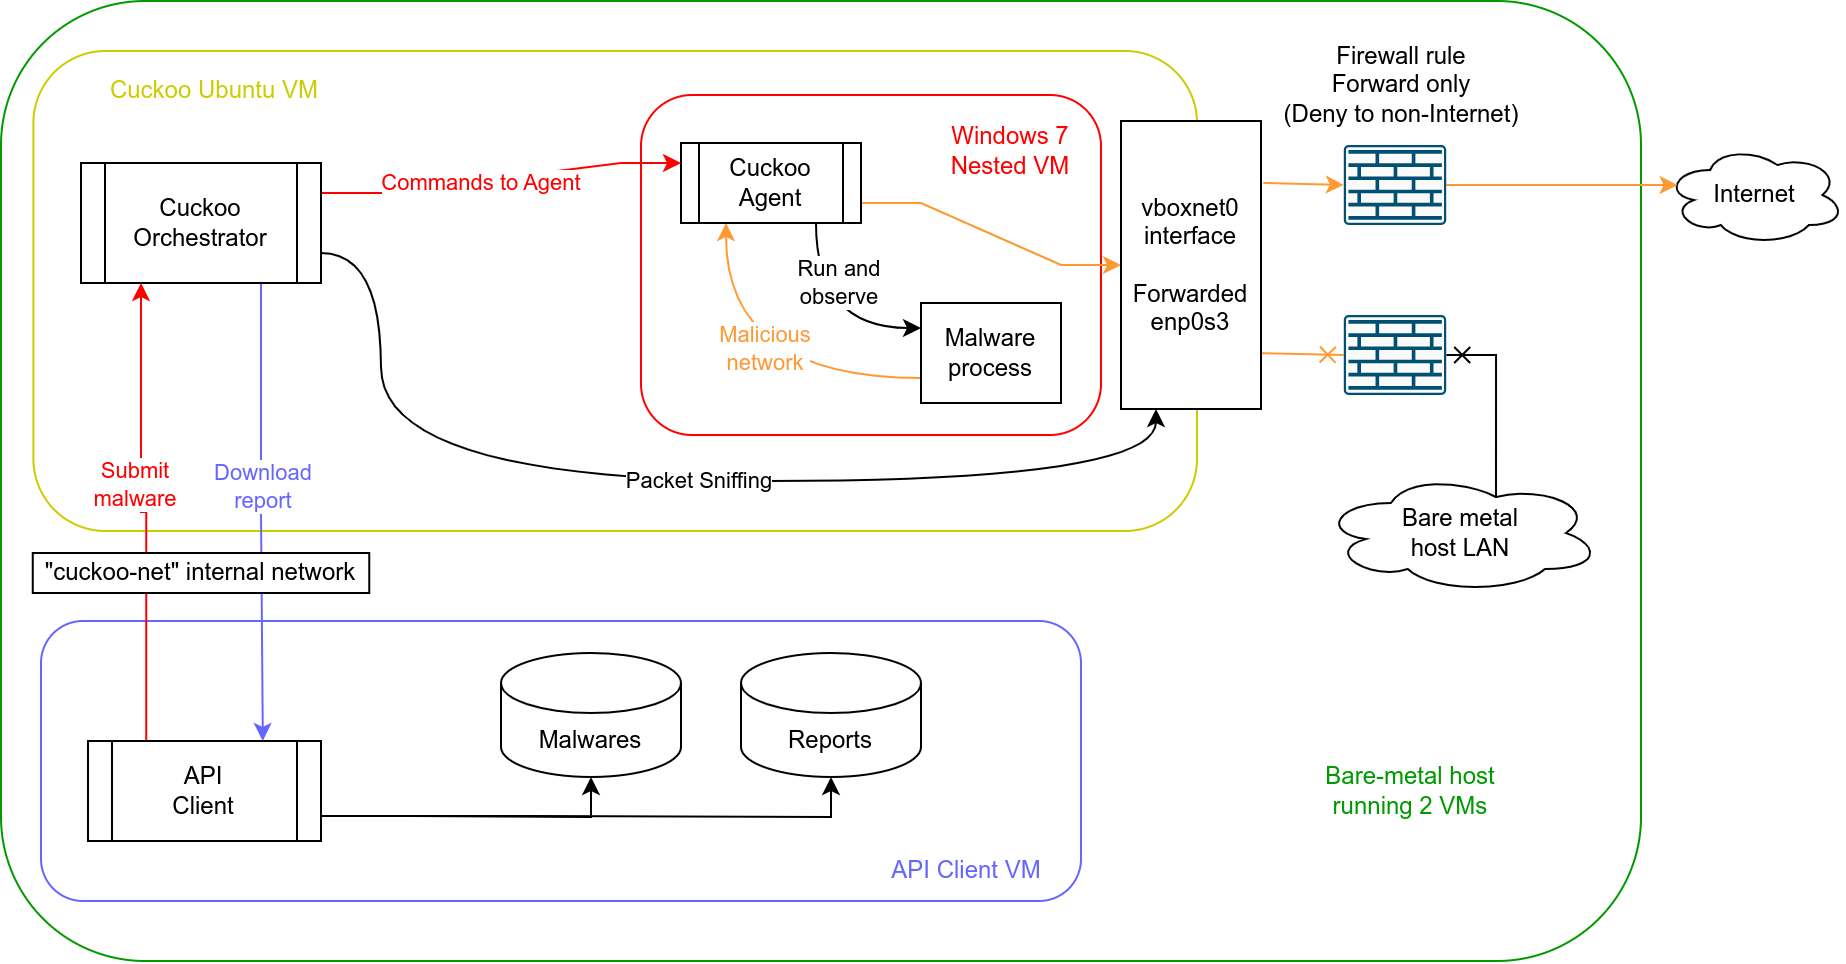
\includegraphics[width=\textwidth]{assets/cuckoo_vms.png}
    \caption{Architettura dell'infrastruttura di analisi dinamica}
    \label{fig:cuckoo_vms_architecture}
\end{figure}

\subsection{Installazione e configurazione}
\label{chap:cuckoo-installation-configuration-services}
Una volta delineato lo schema di ciò che si vuole ottenere e il software alla base da cui partire, il primo passo è la sua installazione e configurazione. Non trattandosi di un normale software ma di una serie di componenti complessi da integrare, fin da subito la stessa installazione della sandbox si è dimostrata articolata.

Viene creata la macchina virtuale Cuckoo VM che, siccome conterrà al suo interno sia componenti complessi che altre macchine virtuali, deve avere allocate ingenti risorse. Si è scelto di riservare 8 core CPU e 8GB di RAM a tale scopo, con inizialmente solo 2 istanze delle VM innestate Windows 7. In caso si voglia scalare questo sistema su un server più potente, basterà solamente modificare le risorse allocate nella configurazione di VirtualBox in maniera semplice.

Il primo problema riscontrato è che, data la storicità di Cuckoo, è sviluppato in Python 2, mentre nelle più recenti versioni di Ubuntu la versione di Python di default è la 3, notoriamente non retrocompatibile.
Viene così installato Python 2 manualmente, poi creato un virtual environment (\texttt{virtualenv}) per isolare le dipendenze del progetto dai pacchetti Python installati globalmente nel sistema e rendere il comando \texttt{python} di default un alias della versione 2, quando questo ambiente virtuale è attivato.
Un virtualenv Python è definito dalla Python Enhancement Proposals PEP-405
\footnote{\url{https://peps.python.org/pep-0405/}}
e fornisce gli strumenti per creare ambienti isolati tra loro, aventi ognuno le proprie dipendenze, versione dell'interprete e altre caratteristiche per non rompere il resto del sistema o progetti tra loro incompatibili, come in questo caso.
Per impostare l'uso di una versione diversa da quella di default, si è usato il comando \texttt{virtualenv --python="\$(which python2.7)" VENV\_PATH/.venv}; l'attivazione si realizza con l'esecuzione di \texttt{source .venv/bin/activate} trovandosi all'interno della directory del progetto.

Successivamente alle dipendenze Python, è stato richiesto di installare anche tutta una serie di servizi esterni.
Il primo è chiaramente VirtualBox internamente alla VM stessa, per procedere con la virtualizzazione innestata.
Poi sono venuti tutti i servizi necessari per il funzionamento dell'Orchestrator di Cuckoo, come il database PostgreSQL, MongoDB per la cache ed ElasticSearch per la correlazione dei dati. La scelta migliore per questi è stata la realizzazione di un file \texttt{docker-compose.yml} con tutti i servizi necessari e loro configurazioni (come variabili d'ambiente, mount di file o bind di porte di rete sull'interfaccia di loopback), installando perciò solo Docker e Docker Compose nel sistema, per avere massima compatibilità e minori problemi di setup dei servizi.

Una volta che tutti i servizi accessori sono pronti per essere utilizzati, e dopo aver aggiornato i file di configurazione di Cuckoo per permetterne la raggiungibilità, vanno attivati i servizi di Web interface e REST API.
La prima ci servirà solamente in locale sulla VM stessa, non esposta all'esterno, a fini di debug e per un utilizzo iniziale più semplice. La seconda, al contrario, andrà esposta sulla rete interna \emph{cuckoo-net} per permettere alla VM \emph{API Client} di interagirvi. In questa fase di setup iniziale, viene tutto esposto su ogni interfaccia (bind su \texttt{0.0.0.0}) per facilitarne il debug, poi perfezionato durante l'Hardening (sez. \ref{chap:dynamic-vm-hardening}).

\subsection{Creazione delle VM Windows}
Per quanto concerne le VM innestate con Windows, si è scelto di adoperare la versione 7 del sistema operativo. Questa è ancora molto diffusa, soprattutto in ambito enterprise dove eventuali malware creerebbero maggiori danni, è supportata da Cuckoo allo stato attuale e, infine, ha opzioni per disattivare il maggior numero di funzionalità di sicurezza di Windows, quindi analizzare a pieno tutti i comportamenti che desidererà compiere il malware nell'ambiente di sandbox.

La creazione di una o più istanze del Guest è stata eseguita con \texttt{vmcloak}.
Questo strumento si interfaccia con VirtualBox e consente la creazione di VM in maniera automatizzata e replicabile.

Viene assegnata una quantità di risorse paragonabile a un computer di fascia bassa verosimile. Il disco sarà di 128GB, allocato dinamicamente, con 4 core CPU e 2GB di RAM. Consentità un'esecuzione non eccessivamente limitante, senza sprecare troppe risorse, specialmente se si prevede di aumentare la parallelizzazione, come spiegato nella sez. \ref{chap:dynamic-vm-replication}.

Vengono poi installati al loro interno tutta una serie di strumenti di utilità che ci si aspetterebbe di trovare in un normale PC aziendale o personale. Questa caratteristica potrebbe sembrare superflua ma in realtà gioca un ruolo molto importante assieme alle più avanzate tecniche di anti-VM-detection che vedremo nella sezione \ref{chap:dynamic-anti-vm-detection}:
\begin{itemize}
    \item Serve come prima tecnica superficiale di anti-VM-detection, per cui un malware potrebbe rilevare se ci si trova in un ambiente di test o meno in base alla presenza o assenza di software che la quasi totalità degli utenti reali avrebbe sul proprio computer
    \item Ampia la superficie di attacco possibile sulla macchina Windows, in caso un malware non esegua direttamente il codice che genera danni nel sistema target ma, in maniera più subdola, vada a sfruttare falle di sicurezza presenti in altri programmi che comunemente un utente avrebbe
    \item Permette l'analisi di file diversi da eseguibili, come DOCX con macro non desiderate o PDF con payload specifici
\end{itemize}

Gli specifici software installati sono:
\begin{itemize}
    \item Adobe PDF Reader
    \item DotNet, Java, Flash e Visual C++ Redistributable 2015: per eseguire programmi che richiedono queste runtime
    \item Internet Explorer 11, Google Chrome e Firefox
    \item Modifica dello sfondo da quello di default a uno random
    \item WinRAR
    \item Windows 7 Service Pack 1
    \item Risoluzione dello schermo fissata a 1280x1024
    \item Suite Office
\end{itemize}

Chiaramente, è stato rigorosamente proibita l'installazione delle VirtualBox Guest Additions, che hanno lo scopo di integrare meglio la VM e fornire più servizi, ossia il contrario dell'obiettivo prefissato.

\subsection{Anti-VM detection}
\label{chap:dynamic-anti-vm-detection}
Alcuni malware, per rendere più difficoltosa l'analisi in ambienti controllati, quindi rallentare lo sviluppo di un rilevamento accurato e una conseguente mitigazione, adottano tecniche di VM-detection. Se rilevano di essere sotto analisi, non eseguono affatto il comportamento che svolgerebbero su un ambiente reale, sia non compiendo azioni o compiendone di normali. Un esempio può essere un Trojan che, se sotto analisi, eseguirà regolarmente il programma autentico per cui si camuffa, distruggendo il sistema solo in ambienti reali.

Data la numerosità di queste tecniche, si è reso necessario trovare una PoC che possa eseguirle in maggior numero possibile e restituire un report su quali rilevazioni bisogna intervenire. \emph{Pafish64} è un progetto open source, rilasciato sotto licenza GPLv3 e disponibile su GitHub
\footnote{\url{https://github.com/a0rtega/pafish}},
che ha come scopo proprio ciò di cui necessitiamo in questo stadio.
Procediamo ad eseguire questo test sulle VM realizzate, senza ancora aver adottato alcuna strategia di mitigazione, per individuare dove e come operare. Il risultato, riportato in figura \ref{fig:pafish_standard_vm}, è pessimo: un gran numero di test falliscono, tra cui:
\begin{enumerate}
    \item tutti quelli che verificano la presenza di un potenziale essere umano,
    visualizzando un dialog con un tasto OK e aspettando che qualcuno lo vada a premere
    \item la rilevazione dell'hypervisor VirtualBox che si sta utilizzando
    \item alcuni controlli su aspetti più specifici della CPU
\end{enumerate}

Come prima strategia, si va ad installare nelle VM le DLL fornite da Cuckoo per fare l'injection delle chiamate di sistema che un processo eseguirà per tali rilevamenti, come nascondere alcuni registri di sistema intercettando le syscall \texttt{RegOpenKeyEx}, o eseguire OCR sullo schermo e muovere il mouse di conseguenza, compiendo azioni banali che un utente eseguirebbe con alta probabilità.
Appena impostata la DLL injection, viene ripetuto il test. Il risultato è in figura \ref{fig:pafish_cuckoo} e presenta molti meno risultati negativi.
Tuttavia, non si potrà progredire ulteriormente a causa dell'attuale architettura impostata e della ben maggiore difficoltà che avrebbe la realizzazione di soluzioni di mitigazione più sofisticate, al di fuori dello scopo del progetto qui realizzato.
Infatti, a titolo esemplificativo, notiamo come l'hypervisor ottenuto leggendo i valori forniti dalla CPU (virtuale) sia \emph{VBoxVBoxVBox}, riconducibile a VirtualBox; questo accade perché valori del genere vengono letti dalla macchina su cui la VM Windows 7 esegue, ma nella configurazione realizzata si tratta a sua volta di VirtualBox, per cui la mitigazione risulta inefficace.

Ci si ritiene però altamente soddisfatti del risultato poiché sono pochissimi i test che falliscono, abbassando la probabilità che un malware da analizzare utilizzi proprio quelli. Non può usarne in gran numero poiché sono rilevabili dalla sanbox tra le syscall eseguite, quindi riportate all'analista che può subito dedurre se si tratti di un comportamento lecito o inaspettato.

\begin{figure}[htbp]
\centering
\begin{subfigure}{.5\textwidth}
  \centering
  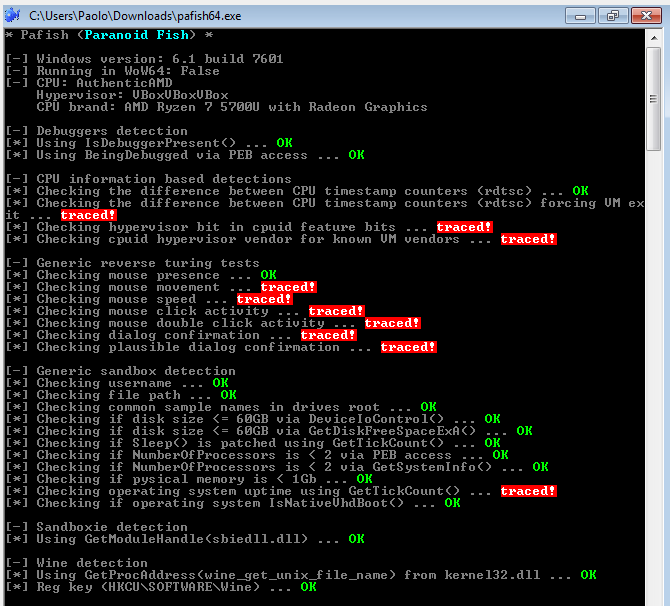
\includegraphics[width=.9\linewidth]{assets/pafish_standard_vm_1.png}
\end{subfigure}%
\begin{subfigure}{.5\textwidth}
  \centering
  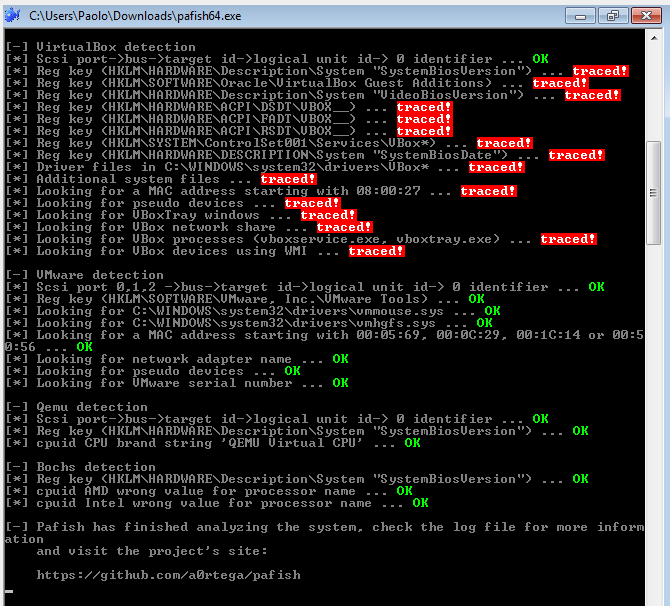
\includegraphics[width=.9\linewidth]{assets/pafish_standard_vm_2.png}
\end{subfigure}
\caption{Pafish eseguito in una classica VM Windows 7}
\label{fig:pafish_standard_vm}
\end{figure}

\begin{figure}[htbp]
\centering
\begin{subfigure}{.5\textwidth}
  \centering
  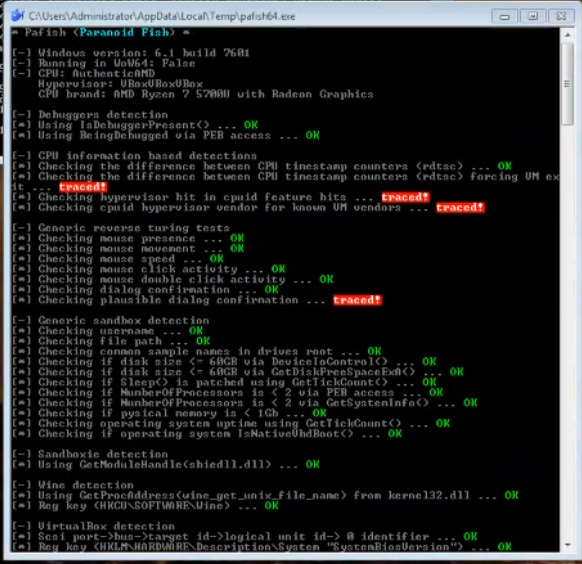
\includegraphics[width=.9\linewidth]{assets/pafish_cuckoo_1.png}
\end{subfigure}%
\begin{subfigure}{.5\textwidth}
  \centering
  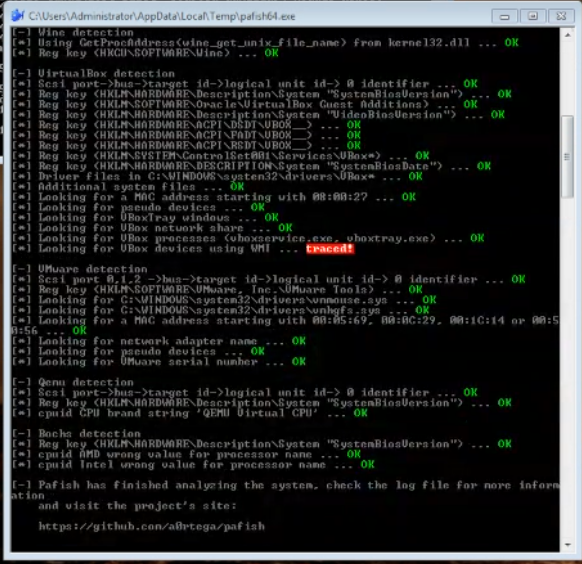
\includegraphics[width=.9\linewidth]{assets/pafish_cuckoo_2.png}
\end{subfigure}
\caption{Pafish eseguito sotto l'analisi di Cuckoo Sandbox}
\label{fig:pafish_cuckoo}
\end{figure}

\subsection{Replicazione VM}
\label{chap:dynamic-vm-replication}
Una volta realizzata una istanza della VM Windows 7, per migliorare la scalabilità del sistema,
quindi permettere che più task possano eseguire in parallelo, 
si devono creare più istanze replicate della macchina virtuale di sandbox.

Per deduplicare la base comune a tutte le istanze, come il sistema operativo e i tool installati, si trasforma il disco virtuale da standard a multi-attach, così da essere connesso a più VM in contemporanea.

A livello di rete si assegna un IP statico a ogni VM, così da permettere a Cuckoo di correlare il traffico verso e da un determinato IP locale, a una specifica VM, quindi a uno specifico task di analisi in corso in un determinato istante di tempo.
Per permettere il forwarding dei pacchetti attraverso questa interfaccia, viene configurata usando il seguente comando:
\begin{minted}{shell}
sudo sysctl -w net.ipv4.conf.vboxnet0.forwarding=1
sudo sysctl -w net.ipv4.conf.enp0s3.forwarding=1
\end{minted}

Infine, si creano le istanze con vmcloak e si eseguono gli snapshot: questi verranno ripristinati subito dopo l'esecuzione di un task di analisi, così da ripartire sempre con lo stesso sistema pulito iniziale e non rischiare che un malware, dopo che infetti la VM, vada a mantenere il controllo della macchina virtuale anche successivamente.

\subsection{Servizi systemd}
Si nota come al boot, tutti i servizi che precedentemente erano funzionanti, debbano essere eseguiti manualmente. Questo passaggio è totalmente da rimuovere per una corretta automazione del processo, e la soluzione migliore in ambito Linux per eseguire servizi al boot è la creazione di \emph{unit di systemd}. Systemd è un sistema di init e gestione dei servizi, ampiamente diffuso nella quasi totalità delle distribuzioni Linux, che deve eseguire con PID 1 (PID 0 è il processo scheduler, parte del kernel) per il corretto funzionamento. I servizi che deve eseguire sono descritti attraverso dei file posti in \texttt{/etc/systemd/system/} chiamati \textbf{unit}.
Come caratteristiche fondamentali, una unit conterrà:
\begin{itemize}
    \item Un nome, dato dal file stesso, e una descrizione per permetterne il riconoscimento in futuro
    \item Uno o più servizi o target da cui dipende, che devono essere avviati prima di esso
    \item L'utente con il quale eseguire
    \item Il comando da lanciare per avviare ed interrompere il servizio
    \item Politiche di restart, che imposteremo ad \emph{always}
    poiché necessitiamo che i vari componenti vengano riavviati automaticamente se dovessero smettere di funzionare
\end{itemize}

Vengono così create le seguenti unit:
\begin{itemize}
    \item \texttt{vboxnet0.service} contiene il comando per creare e avviare preventivamente l'interfaccia di rete
    che useranno Cuckoo e le VM Guest per dialogare e far transitare il traffico di rete da sniffare
    \item \texttt{cuckoo-docker.service} avvia tutti i servizi accessori che Cuckoo
    necessita per il funzionamento, come i database e il resto menzionato in \ref{chap:cuckoo-installation-configuration-services},
    tramite un file Docker Compose
    \item \texttt{cuckoo.service}, che avvierà il demone di Cuckoo una volta che le dipendenze saranno pronte all'uso
    \item \texttt{cuckoo-api.service}, responsabile del server di REST API usato poi dal client esterno a questa VM
    \item \texttt{cuckoo-web.service} risulta utile quando, in fase di testing, si vuole usare una comoda UI per capire il funzionamento
\end{itemize}

\begin{code}
\begin{minted}{INI}
[Unit]
Description=Cuckoo Web Service
Requires=cuckoo.service
After=cuckoo.service

[Service]
User=cuckoo
RemainAfterExit=yes
ExecStart=/home/cuckoo/cuckoo/bin/cuckoo web -H 127.0.0.1 -p 8000
TimeoutStartSec=0
Restart=always

[Install]
WantedBy=multi-user.target
\end{minted}
\label{lst:systemd-unit-example}
\caption{Esempio di systemd unit per il servizio Web}
\end{code}
\bigskip

\begin{figure}[htbp]
\centering
\begin{tikzpicture}[node distance=1.5cm, xscale=2]
  % Nodes
  \node (cuckoo) [ellipse, draw] {cuckoo};
  \node (vbox) [ellipse, draw, below left= of cuckoo] {vboxnet0};
  \node (docker) [ellipse, draw, above left= of cuckoo] {cuckoo-docker};
  \node (api) [ellipse, draw, below right= of cuckoo] {cuckoo-api};
  \node (web) [ellipse, draw, above right= of cuckoo] {cuckoo-web};

  % Edges
  \draw[->] (vbox) -- (cuckoo);
  \draw[->] (docker) -- (cuckoo);
  \draw[->] (cuckoo) -- (api);
  \draw[->] (cuckoo) -- (web);
\end{tikzpicture}
\caption{Grafo delle dipendenze dei servizi systemd aggiunti}
\label{fig:systemd-cuckoo-dependency-graph}
\end{figure}

\subsection{VM Client con CLI}

\subsubsection{Nuovo formato del report}
Differenze, perché è migliore, come si fa il parsing, problemi ancora aperti, etc

\subsection{Hardening}
\label{chap:dynamic-vm-hardening}
Seguire le varie guide, utente custom, rete, etc

\section{Plugin aggiuntivi}

\section{Workflow analisi dinamica}
